% !TEX root = ../Robotik.tex
\chapter{Industrierobotik}
\section{Industrieroboter}
\begin{itemize}
	\item \textbf{Roboterarm} mit Achsen, Gelenken und Antrieben
	\item Steuerung in einem \textbf{Steuerschrank} mit \textbf{Bedienerkonsole}
	\item \textbf{Handsteuergerät}
\end{itemize}

\subsection{Einsatz}
\begin{itemize}
	\item In wohldefinerter Umgebung, definierte Hindernisse, bekannte Umwelt
	\item Größtes Einsatzgebiet in der Automobilindustrie und deren Zulieferern (\textit{Schweißen, Lackieren, Beschichten ...})
\end{itemize}

\subsection{Trends}
\begin{itemize}
	\item Industrie 4.0, KI, IoT
	\item Human-Robot collaboration
	\item Mobile Roboter und einfachere Bedienung
\end{itemize}

\section{Bauform und Komponenten}
\paragraph{Roboterarm}
\begin{itemize}
	\item Armelemente bzw. Glieder die über Bewegungsachsen miteinander verbunden sind.
	\item Ausgleichszylinder $\Rightarrow$ Motoren werden nicht überlastet, geringere Kräfte sind nötig
\end{itemize}

\paragraph{Endeffektor, Hand}
\begin{itemize}
	\item Das Arbeitsorgan $\Rightarrow$ Werkzeug
	\item Üblicherweise wird die Werkzeugspitze \textit{\textbf{Tool Center Point}(TCP)} genannt
\end{itemize}

\paragraph{Fahrzeug}
\begin{itemize}
	\item optional
	\item meist bodengebunden
	\item ein bis drei Freiheitsgrade
	\item Bsp.: Verfahrschlitten
\end{itemize}

\section{Freiheitsgrade}
\subsection{Definition}
Der Freiheitsgrad (DOF) bezeichnet in der Physik die Anzahl der frei wählbaren, voneinander unabhängigen Parameter eines physikalischen Systems, die dessen Zustand eindeutig kennzeichnen.
\begin{itemize}
	\item In der Mechanik drückt der DOF die Möglichkeit aus im Raum voneinander unabhängig Bewegungen auszuführen
	\item Anzahl der Freiheitsgrade drückt die translatorischen und rotatorischen Bewegungsmöglichkeiten eines Körpers aus
	\item Anzahl der Gelenkachsen $\neq$ Anzahl der Freiheitsgrade
\end{itemize}

\section{Bewegungsachsen}
\subsection{Rotatorisch}
\begin{itemize}
	\item Für Drehbewegungen
	\item Freiheitsgrad: 1
\end{itemize}
\begin{figure}[H]
	\begin{center}
		\includegraphics[scale=0.1]{Resources/PNG/Rotatorisch.PNG}
		\caption{Rotatorische Achse}
		\label{fig:PNG/Rotatorisch.PNG}
	\end{center}
\end{figure}

\subsection{Translatorisch}
\begin{figure}[H]
	\begin{center}
		\includegraphics[scale=0.2]{Resources/PNG/Translatorisch.PNG}
		\caption{Translatorische Achse}
		\label{fig:PNG/Translatorisch.PNG}
	\end{center}
\end{figure}
\begin{itemize}
	\item Für Schubbewegungen
	\item Freiheitsgrad: 1
\end{itemize}
\paragraph{Hauptachsen}
\begin{itemize}
	\item Zum Positionieren des Effektors im Raum
	\item Beeinflussen Position des TCP
	\item Rotatorisch oder Translatorisch
\end{itemize}
\paragraph{Nebenachsen}
\begin{itemize}
	\item Kopf- oder Handachsen
	\item Rufen nur kleine Positionsänderungen hervor
	\item Orientierung des Werkzeugs
	\item Meist rotatorisch
\end{itemize}
\subsection{Rotationsgelenk}
Die Drehachse bildet einen rechten Winkel mit den Achsen der beiden angeschlossenen Glieder.
\begin{figure}[H]
	\begin{center}
		\includegraphics[scale=0.6]{Resources/PNG/Rotationsgelenk.PNG}
		\caption{Rotationsgelenk}
		\label{fig:Resources/PNG/Rotationsgelenk}
	\end{center}
\end{figure}
\subsection{Torsionsgelenk}
Die Drehachse verläuft parallel zu den Achsen der beiden Glieder.
\begin{figure}[H]
	\begin{center}
		\includegraphics[scale=0.6]{Resources/PNG/Torsionsgelenk.PNG}
		\caption{Torsionsgelenk}
		\label{fig:Resources/PNG/Torsionsgelenk}
	\end{center}
\end{figure}
\subsection{Revolvergelenk}
Das Eingangsglied verläuft parallel zur Drehachse, das Ausgangsglied steht im rechten Winkel zur Drehachse.
\begin{figure}[H]
	\begin{center}
		\includegraphics[scale=0.6]{Resources/PNG/Revolvergelenk}
		\caption{Revolvergelenk}
		\label{fig:Resources/PNG/Revolvergelenk}
	\end{center}
\end{figure}
\subsection{Kugelgelenk}
Besitzt 3 Freiheitsgrade, wobei die Beweglichkeit stark eingeschränkt ist.
Arbeitsbereich der X- und Y-Achse wird durch die Konstruktion auf unter
180 grad limitiert.
Die Einkerbung an der Vorderseite lässt an dieser stelle einen 90 grad Winkel zu.
\begin{figure}[H]
	\begin{center}
		\includegraphics[scale=0.8]{Resources/PNG/Kugelgelenk.PNG}
		\caption{Kugelgelenk}
		\label{fig:Resources/PNG/Kugelgelenk.PNG}
	\end{center}
\end{figure}
\section{Arbeitsraum}
\paragraph{Definition} Punkte im 3D-Raum, die von der Roboterhand angefahren werden können.
\section{Grundtypen von Industrierobotern}
\subsection{Portalroboter}
\begin{itemize}
	\item Steife Struktur $\Rightarrow$ sehr große Arbeitsräume möglich
	\item Sehr hohe Genauigkeit
	\item Einfache Steuerung in kartesischen Koordinaten
\end{itemize}
\subsection{Horizontal-Knickarmroboter}
\begin{itemize}
	\item \textbf{SCARA}: Selective Compliance Assembly Robot Arm
	\item Aufbau: Ähnlich des menschlichen Arms, horizontaler Gelenkarmroboter
	\item In der Regel 4 Achsen und Freiheitsgrade $f = 4$
	\item Hohe Steifigkeit in vertikaler Richtung
	\item Hohe Geschwindigkeiten möglich
\end{itemize}
\subsection{Vertikal-Knickarmroboter}
\begin{itemize}
	\item Klassischer, universell einsetzbarer Industrieroboter
	\item 4-6 rotatorische Achsen und Freiheitsgrade
	\item Drei Hauptachsen und drei Nebenachsen
\end{itemize}
\subsection{Parallele Roboter}
\begin{itemize}
	\item Bekannt von Flugsimulatoren, Nachbildung der Beschleunigung durch Kippen einer Plattform gegen den Erdbeschleunigungsvektor
	\item Geschlossene Führungsketten mit fest montierten Antrieben
	\item Paralleler Roboter, da die Antriebsachsen parallel auf den Endeffektor wirken
\end{itemize}
\paragraph{Hexapod}
\begin{itemize}
	\item Hohe Stabilität aber geringe Geschwindigkeit
	\item Aus 6 Linearachsen aufgebaut
\end{itemize}
\paragraph{Delta-Roboter}
\begin{itemize}
	\item Schnelle Handhabung
	\item Drei bis vier Gelenkachsen mit stationären Antrieben
	\item Evtl. Erweiterung mit einer 3-Achs Hand
\end{itemize}
\subsection{Leichtbauroboter}
\begin{itemize}
	\item Typ. Massenverhältnis Industrieroboter Last/Eigenmasse: 1:10
	\item DLR Leichtbauroboter III: Last/Eigenmasse = 1:1
\end{itemize}
\section{Effektoren}
\subsection{Endeffektoren}
\begin{itemize}
	\item Arbeitsorgan am Ende eines Roboterarms, mit dem direkt auf ein Werkstück eingewirkt werden kann.
	\item Angebracht an der entferntesten Stelle einer kinematischen Kette
	\item \textbf{Typen}:
	\subitem Werkzeuge
	\subitem Greifer
	\subitem Prüfmittel
	\item  Zustände der Effektoren werden mit Sensoren erfasst.
\end{itemize}
\subsection{Greifersysteme}
Ein Griff muss \textbf{stabil} sein und \textbf{kollisionsfrei} ausgeführt werden können.
Objekt darf nicht im Greifer abgleiten oder sich verschieben.
%Einschränkungen, wo das Objekt nicht gegriffen werden darf, müssen beachtet werden.
\paragraph{Typen}
\begin{itemize}
	\item \textbf{Mechanisch}
	\item \textbf{Vakuum}
	\item \textbf{Magnetisch}
\end{itemize}
\subsection{Greifplanung}
Ein technischer Griff unterteilt sich in die Sequenzen:
\begin{itemize}
	\item Herstellen des Kontakts zwischen Greifobjekt und Greifer
	\item Sichern des Haltens während der Bewegung in allen Richtungen
	\item Genaues Ablegen des Objekts in der Zielposition und in kürzester Zeit
\end{itemize}
\subsection{Greifprinzipien}
\paragraph{Formschlüssiger Griff}
\begin{itemize}
	\item Das Objekt liegt lose zwischen den Greifbacken
	\item Geringe Kräfte auf das Objekt
	\item Positionserhaltung durch passende Geometrie der Greiferbacken
\end{itemize}
\paragraph{Stoffschlüssiger Griff}
\begin{itemize}
	\item Zwischen Greifer und Objekt wirken Kräfte in Form von Klebstoffen oder Flüssigkeitsbrücken
\end{itemize}
\paragraph{Kraftschlüssiger Griff}
\begin{itemize}
	\item Kontakt zwischen Greifer und Objekt durch Punkt- oder Flächenkräfte
	\item Reibkräfte, Vakuum oder Magnetkräfte
	\item Aneinander pressen, so dass die Reibungskräfte ein Verschieben der Bauteile gegeneinander verhindern
\end{itemize}
\section{Antrieb}
\subsection{Antriebsarten}
\begin{itemize}
	\item Antrieb muss Kräfte und Momente durch das Gewicht der Roboterarme und der Objekte im Effektor kompensieren
	\item Antrieb besteht aus Motor, Getriebe und Wegmesssystem
	\item Drei Antriebsarten:
	\subitem pneumatisch
	\subitem hydraulisch
	\subitem elektrisch
\end{itemize}
\section{Sensor}
Umwandeln einer mechanischen, physikalischen oder chemischen Größe in ein Signal.
Gegenteil eines Aktors.
\subsection{Interne Sensoren} Erfassen interner Zustände des Roboters
\begin{itemize}
	\item Weg- und Winkelmessung
	\item Geschwindigkeit
	\item Batteriespannung
\end{itemize}
%TODO Seite 36/99

\subsection{Externe Sensoren}
Erfassen von Eigenschaften aus der Umwelt des Roboters.

\paragraph{Passive Sensoren}
Keine störenden Einflüsse in der Umwelt, dafür aber ungenau und
umgebungsabhängig

\paragraph{Aktive Sensoren}
Genaue Messungen unter wohldefinierten Bedingungen dafür aber evtl. störende
Einflüsse

\section{Kinematik}
\paragraph{Definition}
Die Kinematik beschreibt nur wie sich ein Körper bewegt und wird daher auch als Bewegungsgeometrie bezeichnet.

\subsection{Kinematikmodul}
\begin{itemize}
	\item Das Kinematikmodul ist für die Positionierung der Gelenke
	\item Grundaufgaben
	\subitem \textbf{Vorwärtsrechnung}: Angeben der Gelenkwinkel durch den Benutzer
	\subitem \textbf{Rückwärtsrechnung}: Angeben der Pose durch den Benutzer, die der Roboter dann anfährt
	\subitem Teachen von Punkten und Bahnen
\end{itemize}
\subsection{Steuerung und Regelung von Industrierobotern}
\begin{itemize}
	\item Robotersteuerung = Hard- und Software zum korrekten Ansteuern des Manipulators
	\item Zwei Komponenten: Bewegungssteuerung und Gelenkregelung
	\subitem Steuerung von Effektoren, Berechnung, Steuerung und Überwachung (\textbf{\textit{Bewegungssteuerung}})
	\subitem Regelung von Position, Geschwindigkeit und Beschleunigung (\textbf{Gelenkregelung})
\end{itemize}
\paragraph{Anforderung an die Regelung}
\begin{itemize}
	\item Möglichst schnelle Armbewegung
	\item Kein Abdriften im Ziel
	\item Kein Überschwingen in Kurven oder im Ziel
\end{itemize}
\subsection{Punkt-zu-Punkt Bewegung}
Beschreiben einer undefinierten Bahn, die aber bei jeder Wiederholung identisch sein wird.\\
Schnellste Bewegung zwischen zwei Punkten\\
\textbf{Asynchrone PTP}: Vollständig unabhängiges Verfahren; Achsen erreichen zu verschiedenen Zeiten das Ziel\\
\textbf{Synchrone PTP}: Leitachse = Achse mit größter Bahndauer; Geschwindigkeit der anderen Achsen werden so vermindert, dass alle Achsen gleichzeitig im Ziel angekommen; Ziel: Reduktion der mech. Belastung\\
\textbf{Vollsynchrone PTP}: Gleiche Bahn-, Beschleunigungs- und Bremszeiten für jedes Gelenk.
\paragraph{Linearbewegung}
\begin{itemize}
	\item Angabe von Anfangs- und Endpunkt
	\item Kürzeste Verbindung von zwei Punkten, aber nicht die Schnellste.
\end{itemize}
\paragraph{Kurvenbahn}
\begin{itemize}
	\item Angabe von Anfangs-, Zwischen- und Endpunkt
	\item 3 Stützpunkte, die exakt angefahren werden, beschreiben eine eindeutige Kurvenbahn.
	\item Exakte Kreisbahn kann problemlos beschrieben werden
\end{itemize}
\subsection{Überschleifen}
\begin{itemize}
	\item Mechanischer Verschleiß wird verringert
	\item Reduktion des Energieverbrauchs
\end{itemize}
\paragraph{Geschwindigkeitsüberschleifen}
Das Verfahren zum nächsten Bahnsegment wird erst begonnen, wenn eine definierte Geschwindigkeit überschritten wird.
\paragraph{Positionsüberschleifen}
Das Verfahren zum nächsten Bahnsegment wird erst begonnen, wenn eine definierte Entfernung zum Zwischenpunkt unterschritten wird.
\paragraph{Positioniergenauigkeit}
Abweichung der Ist-Position von der Soll-Position: Zielsicherheit; absolutes Genauigkeitsmaß
\paragraph{Wiederholgenauigkeit}
Streuung der Ist-Position bei mehrmaliger Anfahrt aus derselben Richtung; relatives Genauigkeitsmaß.
\begin{figure}[H]
	\begin{center}
		\includegraphics[scale=0.6]{Resources/PNG/Wiederholungsgenauigkeit.PNG}
		\caption{Absolut- vs. Wiederholgenauigkeit. A = schlechte AG, B = gute AG, C = schlechte WG, D = gute WG $\Rightarrow$ Kombination aus B und D}
		\label{fig:PNG/Wiederholungsgenauigkeit.PNG}
	\end{center}
\end{figure}
\subsection{Programmierung}
\paragraph{Direkte Verfahren - Online Programmierung}
\begin{itemize}
	\item Teach-In Verfahren
	\item Play-back Verfahren; Programmierer fährt eine Bahn ab, die dann vom Roboter wiederholt wird;
	\item Master-Slave System; Bediener führt einen Masterarm; Bewegung wird vom Slave simultan kopiert
	\item CAD-Basiert
\end{itemize}
\paragraph{Indirekte Verfahren - Offline Programmierung}
\begin{itemize}
	\item Textuelle Programmierung
	\item Graphische Simulation auf Basis CAD
	\item Akustische Programmierung, daher Sprachsteuerung
	\item Aufgabenorientierte Programmierung; Roboter kann Aufgaben erledigen; Programmierer startet Aufgaben
\end{itemize}
\section{Kinetic - Berechnungen}
\subsection{Rotationsmatrizen}
\begin{figure}[H]
	\begin{center}
		\includegraphics[scale=0.5]{Resources/PNG/Rotationsmatrizen.PNG}
		\caption{}
		\label{fig:PNG/Rotationsmatrizen.PNG}
	\end{center}
\end{figure}
\paragraph{Umwandlung ZYX-Euler Winkel in Quaternionen und zurück}
\begin{figure}[H]
	\begin{center}
		\includegraphics[scale=0.7]{Resources/PNG/rotationsmatrizen-quaternionen.PNG}
		\caption{}
		\label{fig:PNG/quaternionen-rotationsmatrizen.PNG}
	\end{center}
\end{figure}
\begin{figure}[H]
	\begin{center}
		\includegraphics[scale=0.7]{Resources/PNG/zyx-euler-quaternionen.PNG}
		\caption{}
		\label{fig:PNG/zyx-euler-quaternionen.PNG}
	\end{center}
\end{figure}
\paragraph{Euler Winkel}
\begin{figure}[H]
	\begin{center}
		\includegraphics[scale=0.4]{Resources/PNG/euler-winkel.PNG}
		\caption{}
		\label{fig:PNG/euler-winkle.PNG}
	\end{center}
\end{figure}
Die Pose des Effektors besteht aus:
\begin{itemize}
	\item XYZ-Koordinaten
	\item Orientierung (z.B. im Euler Format)
\end{itemize}
\paragraph{Homogene Transformation}
//TODO
\subsection{Vorwärts Transformation}
\paragraph{Bestimmung der Position und Orientierung des Endeffektors anhand der Achswinkel}
\begin{figure}[H]
	\begin{center}
		\includegraphics{Resources/PNG/arm-endeffektor.PNG}
		\caption{Franzkescher 3-Achs Roboter}
		\label{fig:PNG/arm-endeffektor.PNG}
	\end{center}
\end{figure}
Annahmen:
\begin{itemize}
	\item $XYZ_0$ liegt auf $XYZ_1$
	\item Die $z_i$-Achse verläuft entlang der Gelenkachse
	\item Die $x_{i-1}$ entlang der Normalen zwischen $z_{i-1}$ und $z_i$
	\item Die Koordinatensysteme werden seriell transformiert
	\item $^0T_3 = ^0T_1 \times ^1T_2 \times ^2T_3$
\end{itemize}
\subsection{Modifizierte Denavit-Hartenbert Transformation}
TODO Really?
\subsection{Inverses kinematisches Problem}
Es gibt mehrere Achsstellungen, die zur gleichen Pose führen würden.
\subsection{Bestimmung der Achswinkel anhand der Position und Orientierung des Endeffektors}
\begin{itemize}
	\item Bei Robotern mit mehr als sechs Freiheitsgraden ist jede Stellung mehrdeutig.
	\item Es muss geprüft werden, ob eine gewünschte Position erreichbar ist:
	\subitem Stellung nicht erreichbar, da Punkt im Raum zu weit entfernt ist.
	\subitem Unzulässige Positionen, die außerhalb eines zulässigen Achsbereichs liegen
	\subitem Kollision mit Objekt
	\item Singularitäten: Berechnung der Achsstellungen nicht möglich
	\subitem \textbf{Konfigurationssingularität} Beispielweise kann die Drehung einer Achse durch eine andere kompensiert werden.
	Daher Abhilfe durch Vermeidung von 180$\deg$ Stellungen.
	\subitem \textbf{Bewegungssingularität} Beispielweise müsste beim Verfahren durch einen Punkt eine Achsdrehung mit unendlich hoher Geschwindigkeit erfolgen.
\end{itemize}
\paragraph{Algebraische Methoden}
Finden von passenden Gleichungssystemen für jedes Gelenk, beispielsweise der Form:
%TODO Format math
	$A cos(\theta_i) + B sin(\theta_i) + C = 0$
	$A sin(\theta_i) - B cos(\theta_i) + D = 0$
\paragraph{Geometrische Methoden}
Lässt sich in der Robotergeometrie ein Punkt finden, an dem Position und Orientierung getrennt betrachtet werden können.
\begin{figure}[H]
	\begin{center}
		\includegraphics[scale=0.5]{Resources/PNG/rueckwaertsrechnung.PNG}
		\caption{}
		\label{fig:PNG/rueckwaertsrechnung.PNG}
	\end{center}
\end{figure}
\paragraph{Vorraussetzungen für die Anwendung dieser Methoden}
\begin{itemize}
	\item drei aufeinander folgende, sich in einem Punkt schneidende Rotationsachsen
	\item drei aufeinander folgende parallele Rotationsachsen (z.B. SCARA)
\end{itemize}
\paragraph{Numerische Methoden}
\begin{itemize}
	\item Berechnung der Achstellungen mit Hilfe von Näherungsverfahren
	\item Von einem Startpunkt müssen die Koordinaten und Gelenkkoordinaten bekannt sein
	\item Mit Hilfe der \textbf{Jacobi-Matrix} lässt sich anschließend die Gelenkkonfiguration eines naheliegenden Punktes bestimmen
	\item Verfahren zur Rückwärtsrechnung in Echtzeit eher ungeeignet
\end{itemize}
\subsection{Koordinatensysteme}
Alle Koordinatensysteme werden als kartesische Rechtssysteme angenommen.
\begin{itemize}
	\item Weltkoordinaten $\Rightarrow$ Fest mit der Welt verbunden
	\item Basiskoordinaten $\Rightarrow$ Fest mit dem Sockel des Roboters verbunden.
	\item Handflanschkoordinaten $\Rightarrow$ Relativ zu den Basiskoordinaten
	\item Werkzeugkoordinaten $\Rightarrow$ Relativ zu den Handflanschkoordinaten
	\item Anwenderkoordinaten $\Rightarrow$ Relativ zu Welt- oder Basiskoordinaten
	\item Werkstückkoordinaten $\Rightarrow$ Mit Werkstück verbunden, relativ zu Anwenderkoordinaten
\end{itemize}
\section{Safety}
%TODO Vllt hinzufügen
\section{Roboterprogrammierungen}
\subsection{Programmierung in RAPID}
Ein RAPID Programm besteht aus einem oder mehreren Tasks:
\begin{itemize}
	\item Mindestens ein \textbf{Motion Task}
	\item Eventuell zusätzliche Background Tasks
\end{itemize}
Konfigurationsmöglichkeiten für einen Task
\begin{itemize}
	\item \textbf{Task in foreground}: Der Task wird erst ausgeführt, wenn der Eltern-Task im Zustand Idle ist
	\item \textbf{Type}:
	\subitem NORMAL: Task reagiert auf START/STOP und NOT-Aus
	\subitem STATIC: Läuft bei Neustart an der aktuellen PZ-Position weiter; Reagiert nicht auf START/STOP und NOT-Aus
	\subitem SEMISTATIC: PZ Rücksetzen bei Neustart; Sonst wie STATIC
\end{itemize}
\subsection{Syntax}
\begin{figure}[H]
	\begin{center}
		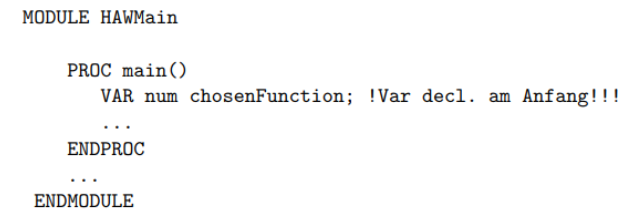
\includegraphics[scale=0.8]{Resources/PNG/Syntax1.PNG}
		\caption{}
		\label{fig:PNG/Syntax1.PNG}
	\end{center}
\end{figure}
\paragraph{Routinen}
können Prozeduren, Funktionen oder Traps sein.
\paragraph{Parameterübergabe}
\begin{itemize}
	\item Reguläre Par: \textbf{PROC \ moveToXY(num \ par1)}
	\item Optionale Par.: \textbf{PROC moveToXY($\backslash$num par1)}
\end{itemize}
\paragraph{Switches}
\begin{itemize}
	\item Switches sind immer optional
	\item Mehrere Switches sind möglich
\end{itemize}
\begin{figure}[H]
	\begin{center}
		\includegraphics[scale=0.9]{Resources/PNG/Syntax2.PNG}
		\caption{}
		\label{fig:PNG/Syntax2.PNG}
	\end{center}
\end{figure}
\subsubsection{Prozedurdeklaration}
\begin{figure}[H]
	\begin{center}
		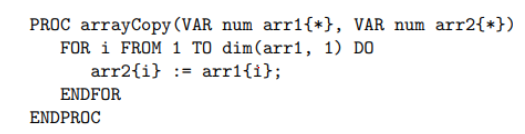
\includegraphics[scale=0.9]{Resources/PNG/Syntax3.PNG}
		\caption{}
		\label{fig:PNG/Syntax3.PNG}
	\end{center}
\end{figure}
\subsubsection{Funktionsdeklaration}
\begin{figure}[H]
	\begin{center}
		\includegraphics[scale=0.9]{Resources/PNG/Syntax4.PNG}
		\caption{}
		\label{fig:PNG/Syntax4.PNG}
	\end{center}
\end{figure}
\subsubsection{Trapdeklaration}
\begin{figure}[H]
	\begin{center}
		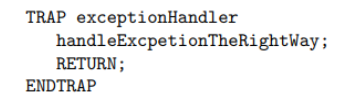
\includegraphics[scale=0.9]{Resources/PNG/Syntax6.PNG}
		\caption{}
		\label{fig:PNG/Syntax6.PNG}
	\end{center}
\end{figure}
\subsubsection{Routinen Aufruf}
\begin{figure}[H]
	\begin{center}
		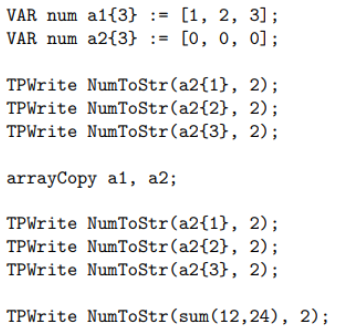
\includegraphics[scale=0.9]{Resources/PNG/Syntax7.PNG}
		\caption{}
		\label{fig:PNG/Syntax7.PNG}
	\end{center}
\end{figure}
\subsubsection{Datentypen}
\begin{itemize}
	\item Jeder Datentyp ist Value- oder Non-Value
	\item Atomarer Datentyp
	\item Zusammengesetzter Datentyp
	\item Alias
	\item Signal - Ausnahme Semi-Value
	\subitem Abfragen Wertbasiert, daher 0,1
	\subitem Initialisierung und Zuweisung: Set, Reset, PulseDO, SetGO
\end{itemize}
\begin{figure}[H]
	\begin{center}
		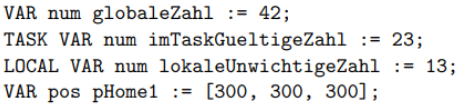
\includegraphics{Resources/PNG/Syntax8.PNG}
		\caption{}
		\label{fig:PNG/Syntax8.PNG}
	\end{center}
\end{figure}
\paragraph{Persistente}
Bsp.: \textit{PERS pos pHome1 := [300, 300, 300];}
\begin{itemize}
	\item Bleiben auch unter folgenden Umständen erhalten
	\subitem Reboot
	\subitem Open, Close, New Programm
	\subitem Start - Move PP to main
	\subitem Start - Move PP to routine
\end{itemize}
\begin{itemize}
	\item Können nur auf Modulebene deklariert werden
	\item Können auf einen Wert initialisiert werden, aber keine erneute Initialisierung bei Reboot
\end{itemize}
\paragraph{Konstanten}
Bsp.: \textit{CONST num euler := 2.7182;}
\subsection{Bewegungsfunktionen}
\paragraph{Move Absolute Joint}
\begin{itemize}
	\item Syntax: MoveAbsJ ToJointPos, Speed, Zone, Tool
	\item Beispiel: MoveAbsJ pHome1, vMax, fine, tool0;
\end{itemize}
\paragraph{Move Joint}
\begin{itemize}
	\item Syntax: MoveJ ToPoint, Speed, Zone, Tool
	\item Beispiel: MoveJ p10, vMax, fine, tool0;
\end{itemize}
\paragraph{Move Linear}
\begin{itemize}
	\item Syntax: MoveL ToPoint, Speed, Zone, Tool
	\item Beispiel: MoveL p10, vMax, fine, tool0;
\end{itemize}
\paragraph{Move Circularly}
\begin{itemize}
	\item Syntax: MoveC CirPoint, ToPoint, Speed, Zone, Tool
	\item Beispiel: MoveC p10, p20, vMax, fine, tool0;
\end{itemize}
\subsection{World Zones}
Es ist nötig den Roboter vor Programmausführung in eine definierte Position zu bringen.
Programmierer ist für die einschränkung der Bewegungen des Roboters verantwortlich, sodass kein schaden entsteht bspweise durch Kollision.
Diese Zone kann sein:
\begin{itemize}
	\item eine Kugel
	\item ein Zylinder
	\item Quader/Box
	\item festgelegte Bereiche bei den Achswinkeln
\end{itemize}
Bei Eintritt des Tool Center Points (TCP) in den definierten Weltzonenbereich kann ein Signal gesetzt werden, das mit Hilfe der Software weiterverwendet werden kann.
Die benötigten Befehle für eine Kugelbereich sind \textit{WZSphDef} und \textit{WZDOSet}.
Das gesetzte Signal ist hier doInHome1, das vorher als IO-Signal definiert wurde.
\begin{figure}[H]
	\begin{center}
		\includegraphics[scale=0.8]{Resources/PNG/robocode1.PNG}
		\caption{}
		\label{fig:PNG/robocode1.PNG}
	\end{center}
\end{figure}
\subsection{Bildschirmein- und -ausgabe}
Die TP-Funktionen bieten die Möglichkeit einer einfachen Bildschirmausgabe und eingabe.
Mögliche Befehle sind \textbf{TPReadDnum}, \textbf{TPReadFK}, \textbf{TPReadNum} und \textbf{TPWrite}.
\subsection{Zeitmessung}
\begin{itemize}
	\item ClkReset - Zurücksetzen / Löschen eines Timers
	\item ClkStart
	\item ClkStop
	\item ClkRead - Auslesen eines (abgelaufenen) Timers
\end{itemize}
\begin{figure}[H]
	\begin{center}
		\includegraphics{Resources/PNG/code1.PNG}
		\caption{}
		\label{fig:PNG/code1.PNG}
	\end{center}
\end{figure}
\subsection{Bewegung relativ}
Um die Anzahl der Teachpunkte möglichst gering zu halten, empfiehlt es sich, wenn möglich, weitere Punkte relativ zu anderen Punkten anzugeben. \\
$\Rightarrow$ Befehl \textbf{Offs}, mit dem die Positionskomponente eines Punktes einfach modifiziert werden kann.\\
VAR robtarget p10 := Offs(pHome, X, Y, Z)
